\documentclass[11pt, oneside]{article}   	% use "amsart" instead of "article" for AMSLaTeX format
\usepackage{geometry}                		% See geometry.pdf to learn the layout options. There are lots.
\geometry{letterpaper}                   		% ... or a4paper or a5paper or ... 
%\geometry{landscape}                		% Activate for rotated page geometry
\usepackage[parfill]{parskip}    		% Activate to begin paragraphs with an empty line rather than an indent
\usepackage{graphicx}				% Use pdf, png, jpg, or eps§ with pdflatex; use eps in DVI mode
\graphicspath{ {Users/hld523/Reports/my-plasma-report/Figures/} }								% TeX will automatically convert eps --> pdf in pdflatex		

\usepackage{amssymb}
\usepackage{amsmath}

%SetFonts

%SetFonts


\title{Brief Article}
\author{The Author}
%\date{}							% Activate to display a given date or no date

\begin{document}
\maketitle
\section{Introduction}
\section{Materials and Methods}

\section{Results}

\subsection{Spatial Resolution of Hydroxyl Radicals}

\begin{figure}
    \centering
    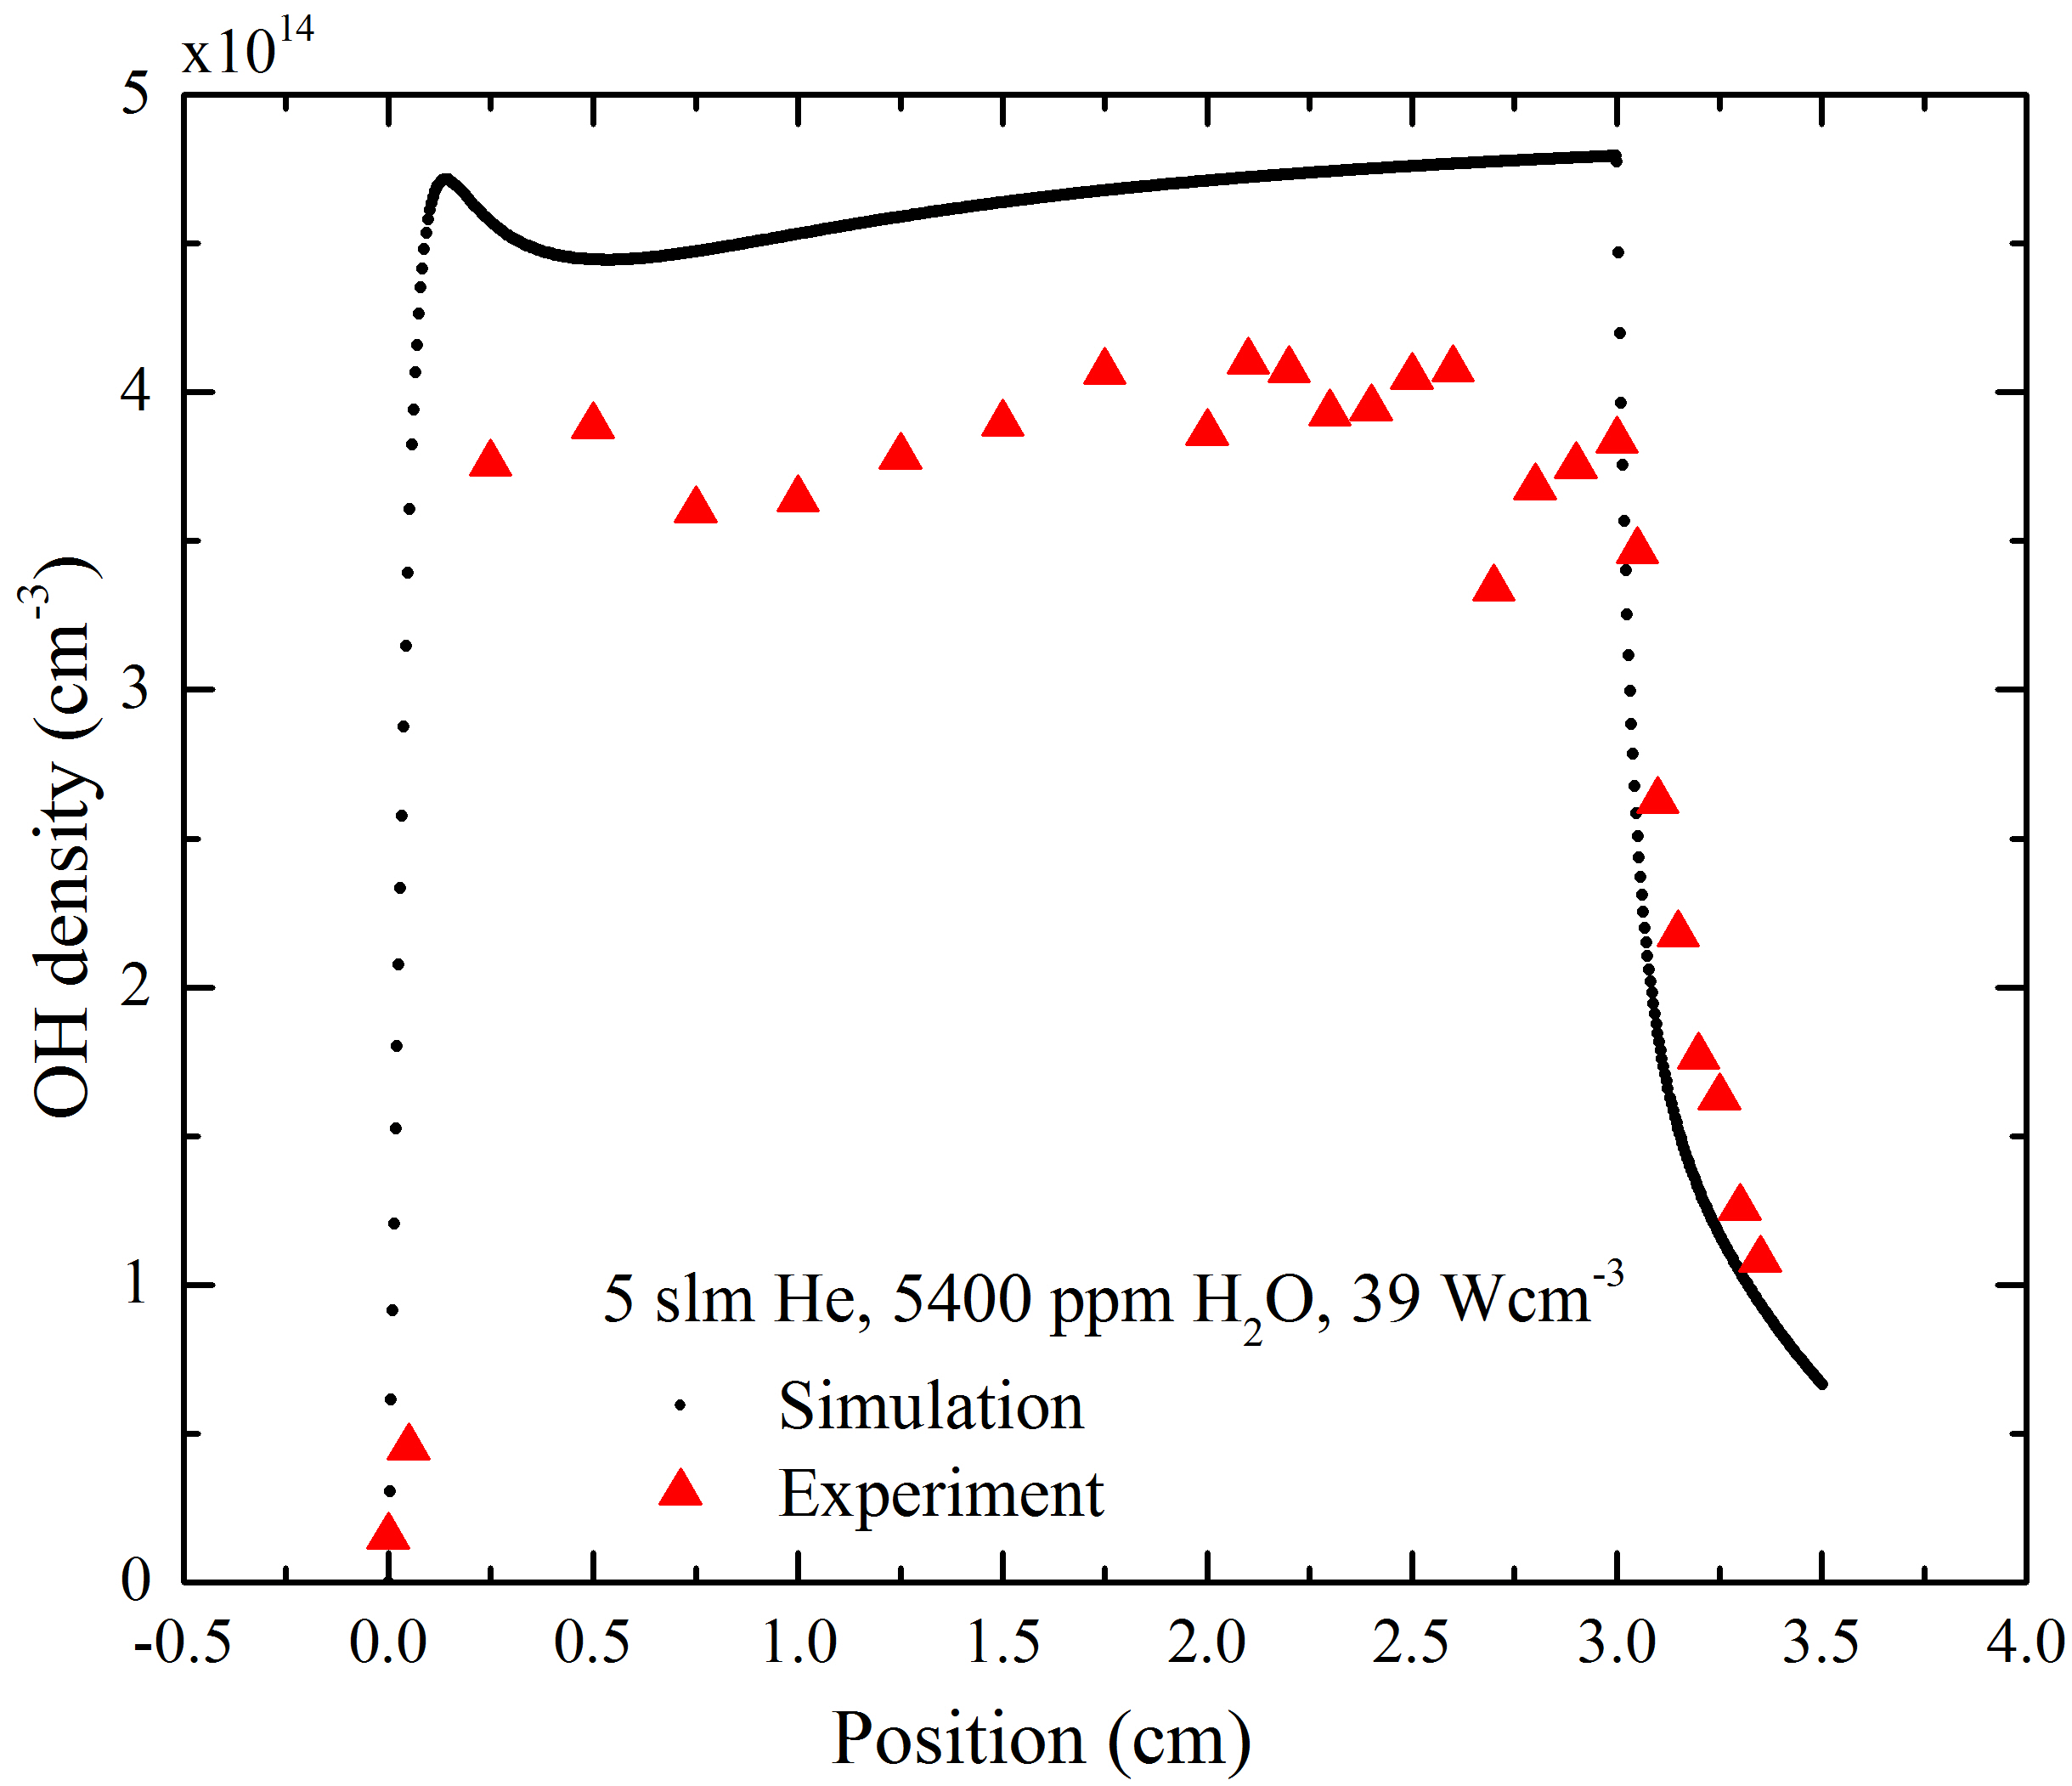
\includegraphics[width=\textwidth]{Figures/OHSpatialwithSim.jpg}
    \caption{Figure showing the effects of distance from gas inlet on the density of hydroxyl radicals in plasma. Absorption spectroscopy was performed at 0.5-1mm intervals along the 30mm length of the electrodes (0-30mm), plus at 0.5mm intervals beyond the end of the plasma region (30.5-33.5mm). This was performed at the maximum power for the plasma before arcing occurs. A total gas flow of 5 slm helium was used with 5400ppm water.}
    \label{fig:SpatialRes}
\end{figure}

\begin{figure}
	\centering
	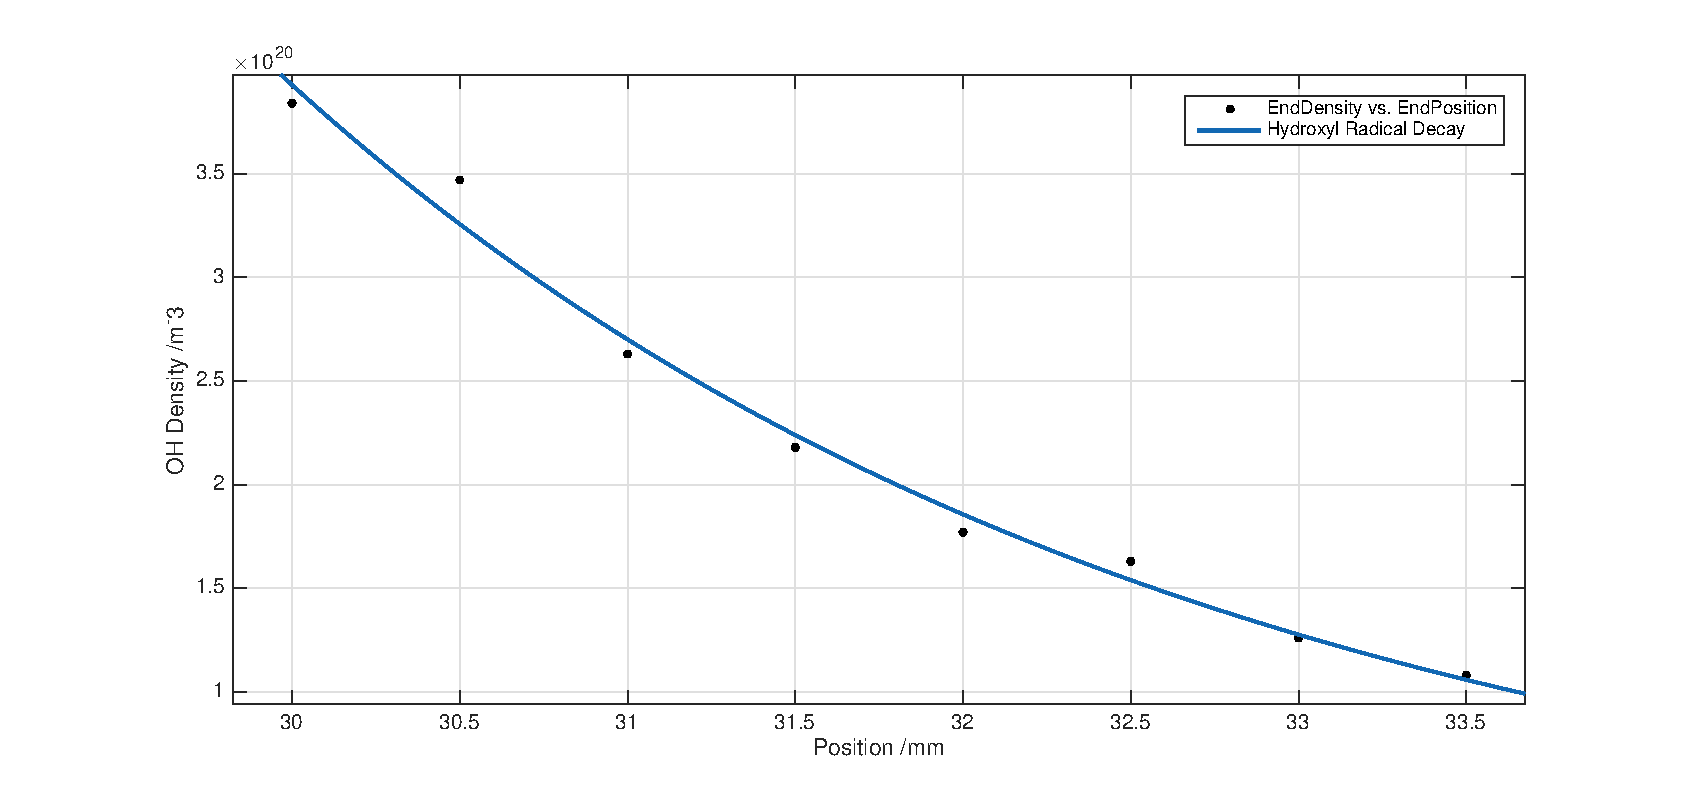
\includegraphics[width=\textwidth]{Figures/OHdecay.eps}
	\caption{Figure showing how the density of hydroxyl radicals falls away exponentially beyond the electrodes. The 30mm point is the end of the electrodes and 33.5mm is the last point where the measurement could be taken before the LED was blocked by the casing of the plasma source.}
	\label{fig:OH decay}
\end{figure}


The aim of this is to show how the distance from the gas inlet, and therefore, position along the 30mm electrode, affects the density of hydroxyl radicals. Figure \ref{fig:SpatialRes}.
It also is able to provide information on the decay rate of hydroxyl radicals at the end of the electrodes.
Also able to compare to simulated data.
Data acquired using a power of Op97 which is the maximum power that can be applied to the plasma before arcing occurs.
\begin{itemize}
    \item Sharp increase from 0-2.5mm, followed by a smaller increase and decrease to give a little hump seen in both the experimental and simulated data. Following this there is an increase in density over the rest of the channel. The change is very small (less than 1 x 1020 m-3)
   
    \item Significant decrease in hydroxyl radical density beyond the end of the electrodes. Distance is not sufficient to allow the density to decrease to the densities seen at the very start of the electrodes. 
        
    \item To interrogate the decrease beyond the end of the electrodes, the measurements were taken every 0.5mm from the end of the channel to the edge of the casing. A curve was then fitted to the data points to see the decay of hydroxyl radicals with distance from the end of the electrodes
    
    \item Have to be careful to say this is the true decay though as the whole casing of the plasma source acts as the grounded electrode so in fact, the ends of the electrodes will still be interacting with the grounded casing around the ends of the electrode.
    
    \item However, very nice exponential decay curve can be drawn for the decay. Half distance (like half life but in distance rather than time!!!) is approximately 1.9mm!
\end{itemize}

Overall, both the experimental and simulated data show a similar trend over the full length of the plasma channel with a sharp increase at the beginning, a small increase and decrease between approximately 2.5 - 7 mm, followed by an overall slight increase in density to the end of the electrodes.
Beyond the electrodes the density seems to decrease quickly with a lifetime of ???????.
This very short lifetime is due to the fact that hydroxyl radicals react very readily with everything and are therefore lost.

\subsubsection{The percentage dissociation is very small}

The degree of dissociation of water to hydroxyl radicals was then investigated... 
This showed that the percentage dissociation (hydroxyl/water *100) was very small.
However, while these numbers seemingly show that only a small amount of the water is dissociating, it may also be that the hydroxyl is recombining with other things and therefore being lost.

\begin{figure}
	\centering
	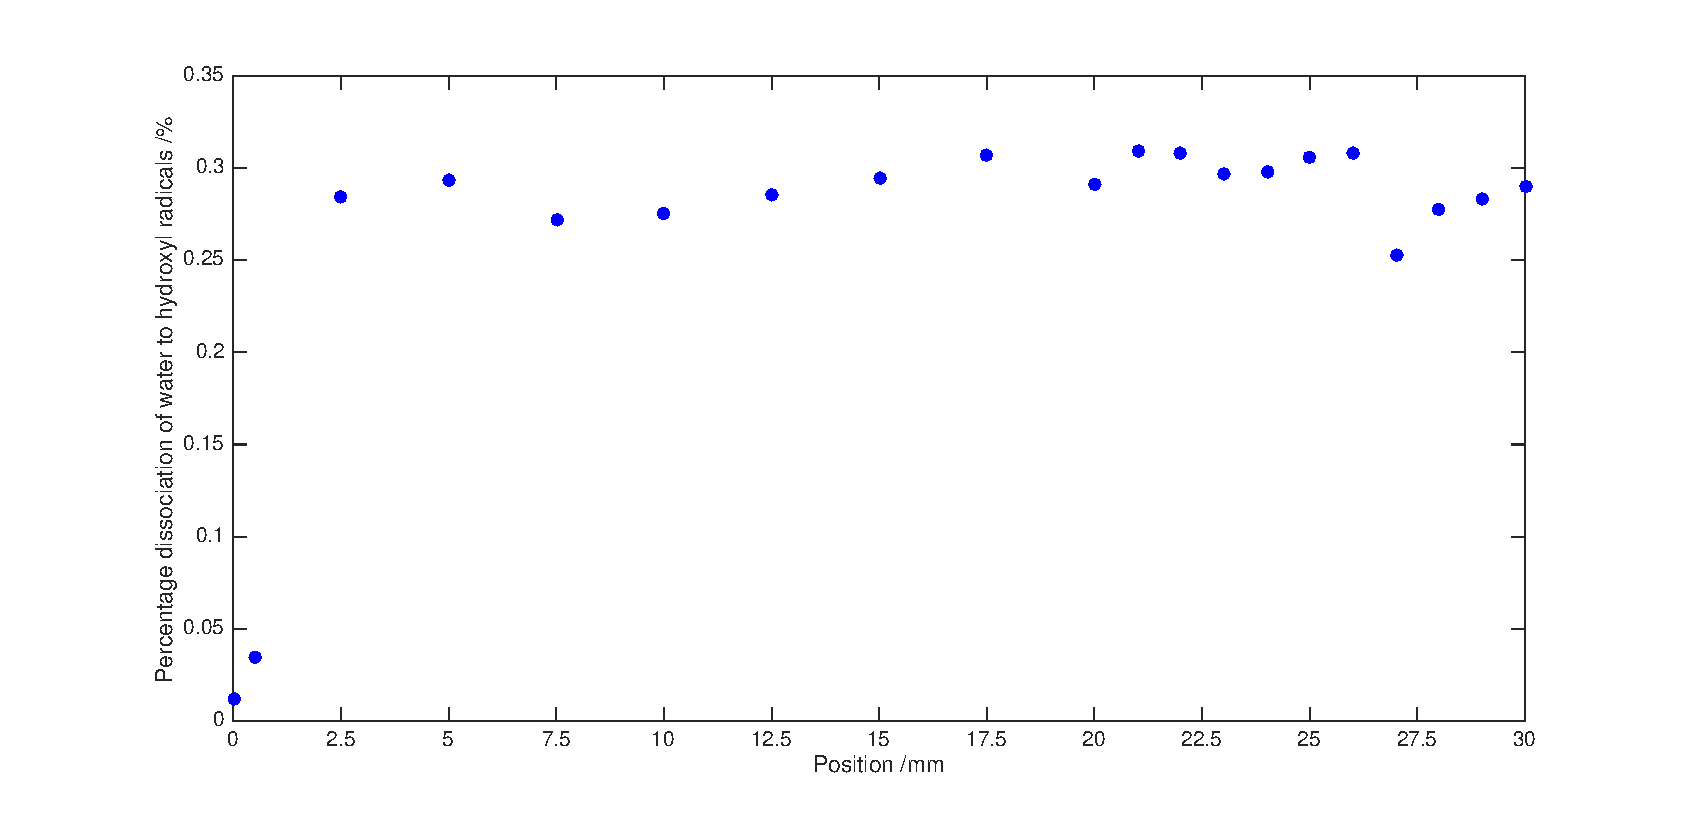
\includegraphics[width=\textwidth]{Figures/SpatialDissociation2.eps}
	\caption{The figure shows the percentage dissociation of water to hydroxyl radicals, calculated as ppm hydroxyl radicals divided by ppm water in, all multiplied by 100. Since the ppm of water stays the same at all positions, the graph shows the same trend as the equivalent density graph.}
	\label{fig:SpatialDissociation}
\end{figure}


\subsection{Increasing the power to the plasma increases hydroxyl radical density}

Following investigation of the spatial resolution of hydroxyl radicals, the effects of power variation were then investigated.
It was of interest to see how varying the power would affect the density of hydroxyl radicals and the percentage dissociation of water to hydroxyl.
The 20mm position was chosen to investigate as at this point, the densities of hydroxyl radical seems to level off slightly. 
The full range of powers for the plasma were tested from ????? (minimum power for sustaining the plasma) to ????? W (maximum power before arcing occurs).

The results of this are shown in figure \ref{fig:PowerVariation}.

\begin{figure}
    \centering
    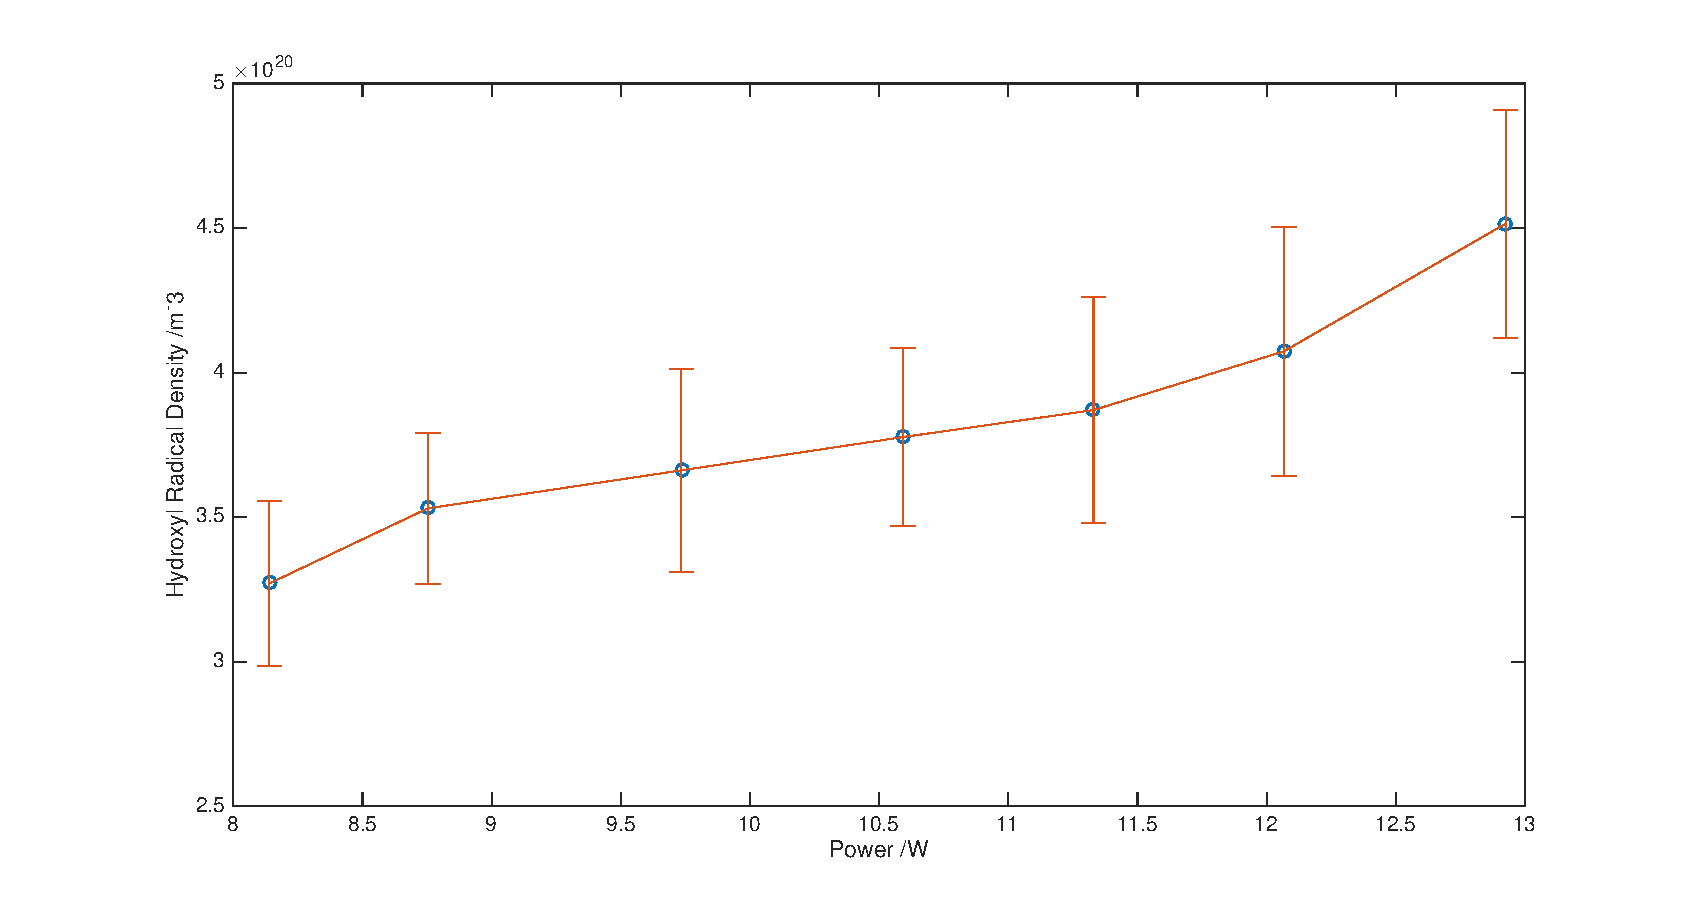
\includegraphics[width=\textwidth]{Figures/PowerVariation.eps}
    \caption{Power increases hydroxyl radical density in the plasma region in a non-linear manner. Absorption spectroscopy was performed at a point 20mm from the gas inlet while power being dissipated in the plasma was varied within the range of ????8.1-12.9W???. Total gas flow to the plasma was kept constant at 5slm helium with 5400ppm water. The experiment was repeated four times. The graph shows the average density for each power and the error bars represent one standard deviation.}
    \label{fig:PowerVariation}
\end{figure}

\begin{itemize}
    \item Densities increase non-linearly from min to maximum power.  Density at min and max power are similar to those seen in spatial resolution data, at least, within the error.
    \item Density range of approximately 3.25 - 4.5 x 10\textsuperscript{20} m\textsuperscript{-3}
    \item Experiment repeated 4 times ? gives indication of expected error of approximately +/- 0.5 x 10\textsuperscript{20} m\textsuperscript{-3}.
\end{itemize}

\subsubsection{Dissociation}

The dissociation of water to hydroxyl radicals was then investigated for this experiment and, once again, the percentage dissociations were extremely small, though they did increase for the increased power. 
Unfortunately, the power cannot be increased any more for this setup before arcing occurs therefore increasing the dissociation would have to be achieved a different way. ?Increasing frequency may be a possibility.

\begin{itemize}
    \item Percentage dissociation increases with increasing power.
    \item Unfortunately, 12.9W is the maximum power achievable before arcing occurs in the plasma. It may be that without increasing the power it is not possible to increase the percentage dissociation. ?Increase frequency.
    \item Percentage is extremely small. This may be due to the very short lifetime of hydroxyl radicals which ultimately become more stable species. While it appears that the dissociation of water to .OH is very small, it may be that the water dissociates to .OH then the .OH is very quickly lost to other species making it undetectable. Would it be possible to measure water in the plasma to see how much is lost/left undissociated?
\end{itemize}

\begin{figure}
    \centering
    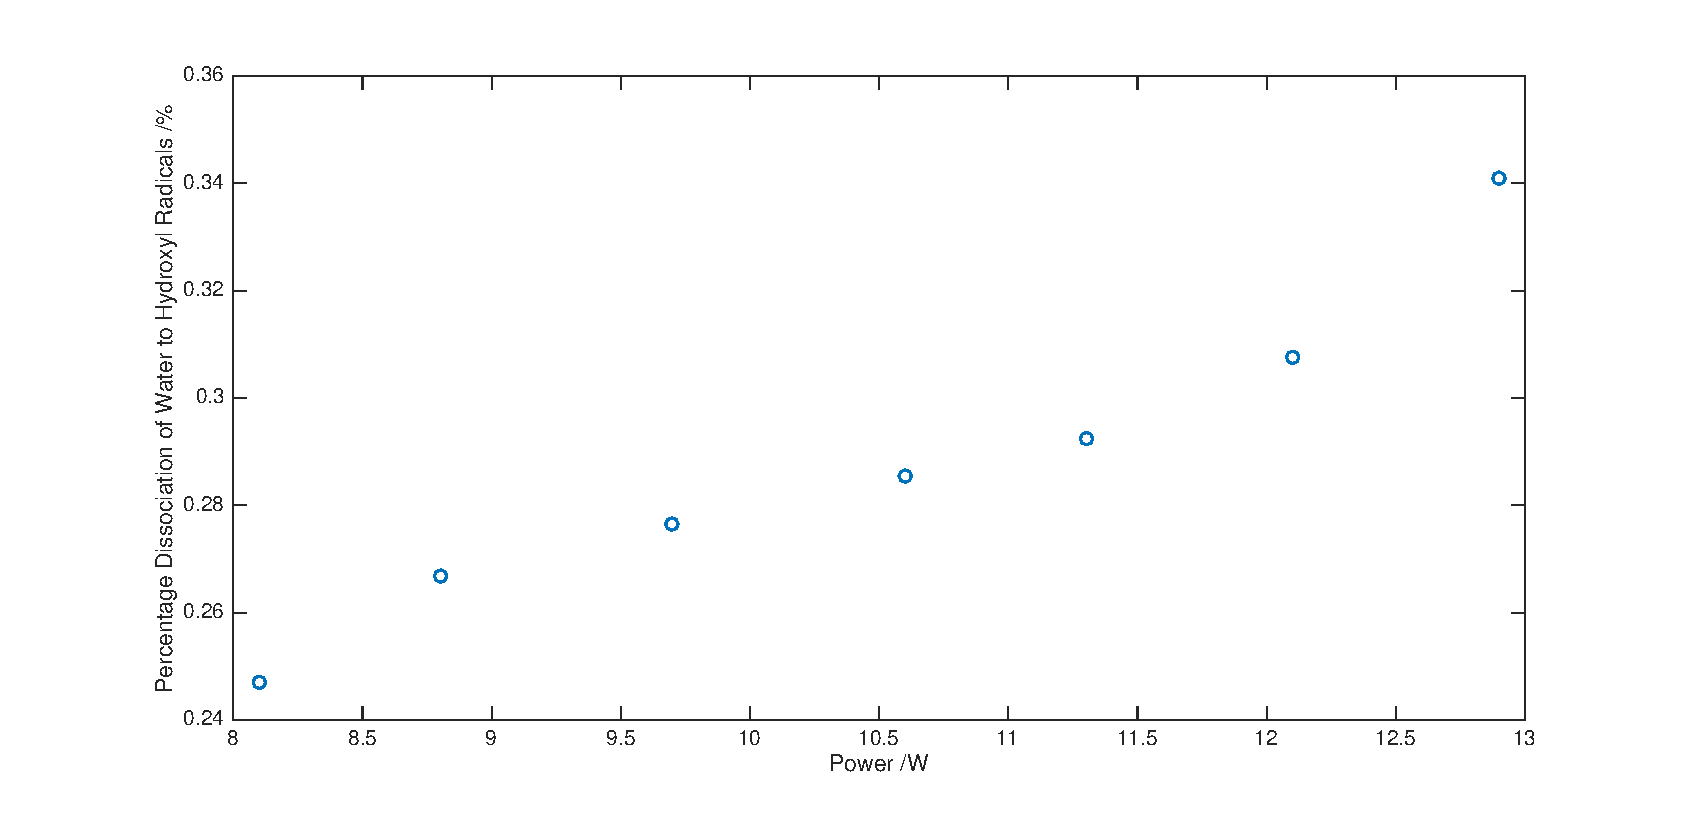
\includegraphics[width=\textwidth]{Figures/PowerDissociation.eps}
    \caption{Percentage dissociation of water to hydroxyl radicals increases with increasing power. Absorption spectroscopy was performed at a point 20mm from the gas inlet. The plasma was operated with a total gas flow of 5slm helium plus 5400ppm water. The percentage dissociation was calculated using the average density of hydroxyl radicals as shown in figure \ref{fig:PowerVariation}. The power range was ??8.1-12.9W??.}
    \label{fig:PowerDissociation}
\end{figure}

\subsection{Increasing the water content of the plasma gas feed increases hydroxyl radical density}

To investigate whether increasing the water being fed to the plasma increases the hydroxyl radical density, the ratio of dry and humid helium entering the plasma channel was altered by changing the proportion of the total 5 slm helium that passed through the bubbler. The range of water concentrations entering the plasma was approximately 2700 - 13400 ppm. The results are shown in figure \ref{fig:BubblerVariation}.

The powers had to be carefully chosen due to the effects of adding in additional molecules into the plasma which can act as energy sinks when they absorb energy to change rotational and vibrational states. 
Therefore, higher water contents require higher powers to ignite as the system becomes less efficient when more molecules are added.
Two different powers were used to investigate the effects of altering the water content. Firstly, ??W was used as this was sufficient to sustain the plasma at high water contents, without causing arcing at low contents. Secondly, the power was increased to see how the density increased at the higher power. 

\begin{figure}
    \centering
    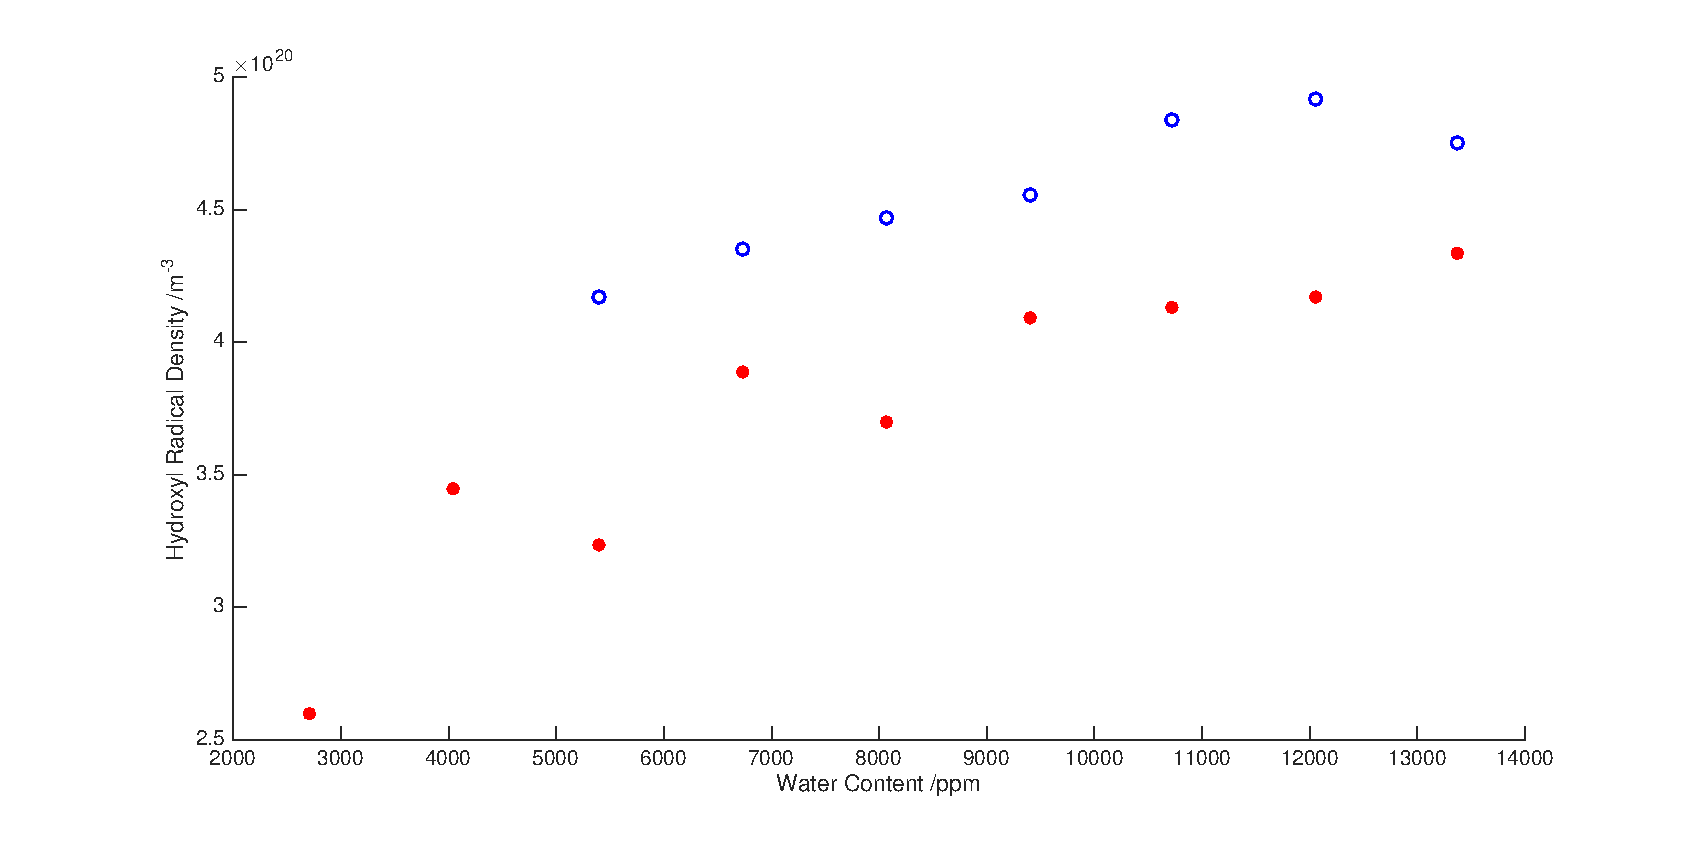
\includegraphics[width=\textwidth]{Figures/BubblerVariation}
    \caption{Increasing the water content of the helium entering the plasma channel increases hydroxyl radical density. Absorption spectroscopy of plasma at 20mm from the gas inlet was performed with different ratios of ?dry? and ?humid? helium entering the plasma channel. A total gas flow of 5 slm was maintained throughout. The range of water contents of the gas feed was approximately 2700 - 13400 ppm. The powers used were ??10.6W?? and ??12.9W??}
    \label{fig:BubblerVariation}
\end{figure}

\begin{itemize}
    \item Increasing the water content in the feed gas to the plasma increases the hydroxyl radical density
    \item The same trend is seen at both the lower and higher powers, though the densities are consistently higher at the higher power as expected. 
\end{itemize}

\subsubsection{Dissociation}

Look at how percentage dissociation changes with amount of water in plasmas. Figure \ref{fig:BubblerDissociation}.

\begin{figure}
    \centering
    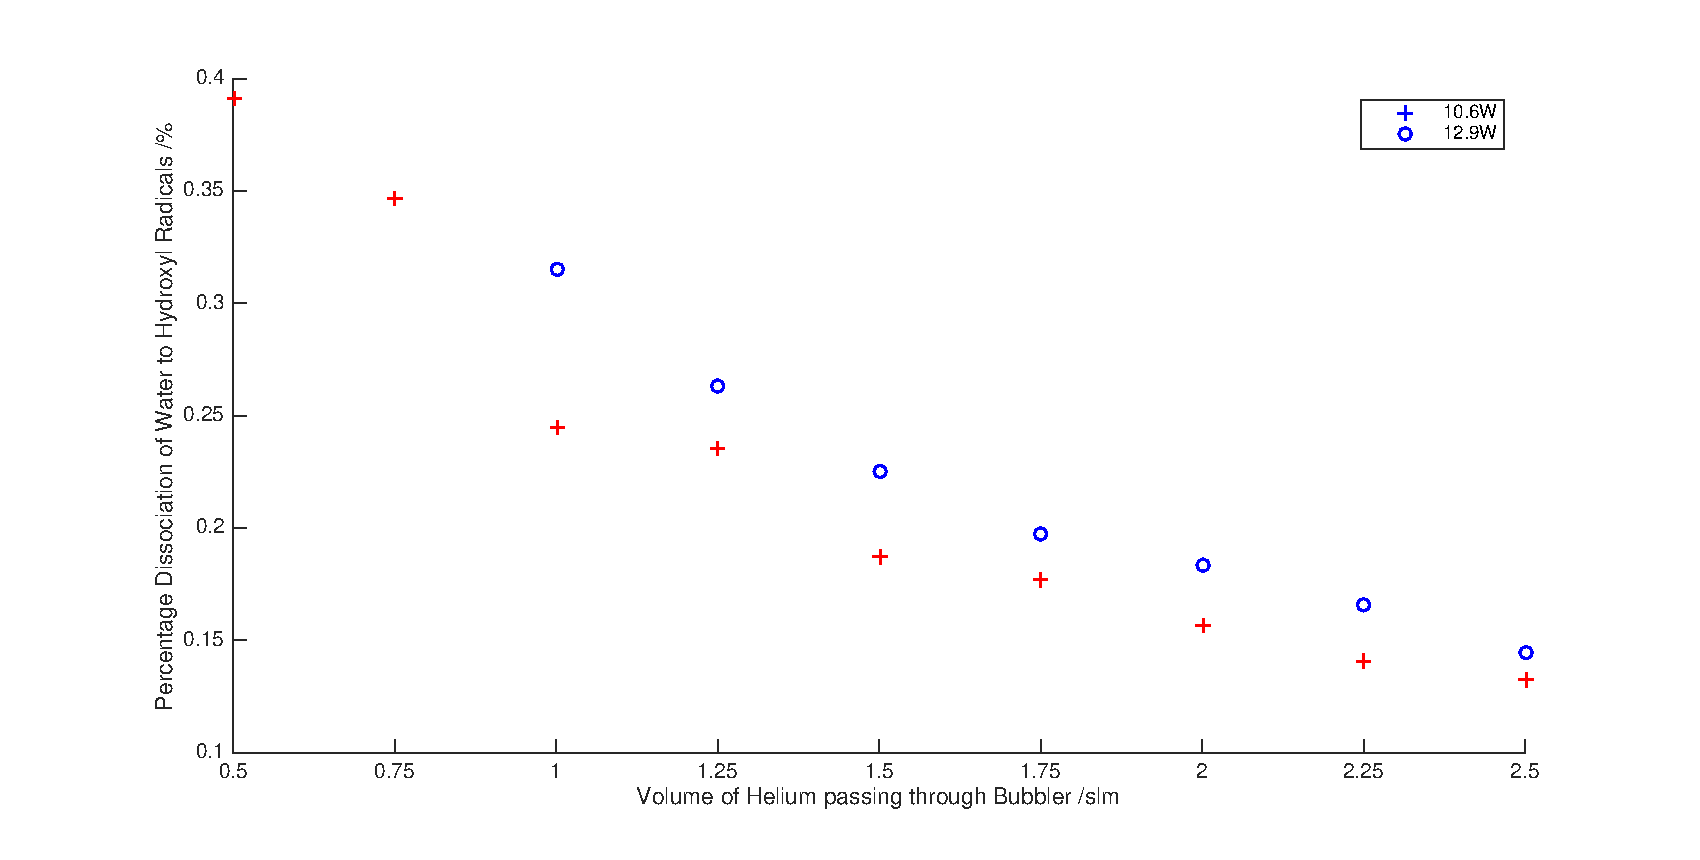
\includegraphics[width=\textwidth]{Figures/BubblerDissociation.eps}
    \caption{The percentage dissociation of water to hydroxyl radicals decreases as the water content increases. Absorption spectroscopy was carried out at a point 20mm from the gas inlet. The plasma was operated with a total of 5slm helium with water contents of 2700 - 13400 ppm. The experiment was repeated at two different powers of ??10.6 and 12.9W??.}
    \label{fig:BubblerDissociation}
\end{figure}

\begin{itemize}
    \item Percentage dissociation decreases with increasing water content, despite the density of hydroxyl radicals increasing (see figure \ref{fig:BubblerVariation}). However, the water content increases more than the density, therefore the ratio of hydroxyl radical to water still decreases.
    \item The dissociation is higher for the higher power than the lower power, as would be expected. 
    \item Dissociation may also decrease due to the increase in energy absorption by molecules. The increase in water content means that more of the energy in the plasma system can be absorbed by the molecules in rotationally and vibrationally excited states. Could add oxygen into the feed gas. In theory, oxygen addition could increase hydroxyl radical density as, when water dissociates, there is a spare hydrogen which could combine with oxygen to form hydroxyl. However, this may have the opposite effect because, once again, a molecule is being added which could contribute further to the absorption of energy from the system. The oxygen would also require energy to be atomised before it could form .OH with the spare hydrogen from water.
\end{itemize}




\section{Discussion}



\end{document}  